\section{复数}
复数的引入源自解三次代数方程的负数平方根问题 。在实数集中,一元二次次方程 $x^2 + 1 = 0$ 无解。
如果,令 $i^2=-1$,称为虚数单位(Imaginary Unit),定义一个全新的数集——复数集,那么任何一个代数方程在复数集中都有解,并且解的个数恰好等于方程的次数,该结论称为代数基本定理。

\begin{theorem}[代数基本定理 Fundamental Theorem of Algebra]
    每一个次数为 $n$ 的非零单变量复系数多项式 $P(z)=a_nz^n + a_{n-1}z^{n-1} + \cdots + a_1z + a_0,\ a_n\neq 0$ 在复数域上恰有 $n$ 个根(重根按重数计算)。
\end{theorem}

\vspace{1em}

\subsection{复数的定义}

\begin{definition}[复数 Complex Number] 有序对 $(a,b)\in\mathbb{R}^2$ 记为 $a+bi$,其中,
    \begin{enumerate}
        \item 约定:$i^2 = -1$;
        \item 等于关系:$a+bi = c+di \Leftrightarrow a=c \land b=d$;
        \item 等价类:$[a+bi]_{=} = \{(c,d)\in\mathbb{R}^2 : a+bi = c+di\}$;
    \end{enumerate}
    称 $\mathbb{R}^2$ 关于 $=$ 关系的商集 $\mathbb{R}^2/_{=}= \{[a+bi]_{=} : a+bi\in\mathbb{R}^2\}$ 为复数集,记为 $\mathbb{C}$。复数集中的元素称为复数。
\end{definition}

\begin{note}
    复数同样是一个等价类,但集合中只有一个有序对 $(a,b)$,所以可以直接用 $a+bi$ 来表示复数。
    在复数中,实数 $a$ 称为复数的实部(Real Part),记为 $\Re(a+bi)=a$;实数 $b$ 称为复数的虚部(Imaginary Part),记为 $\Im(a+bi)=b$。
    全体实数可以嵌入到复数集中,即 $\forall a\in\mathbb{R}$,有 $a =a+0i \in \mathbb{C}$。
\end{note}

\vspace{1em}

\begin{definition}[复数的加法与乘法 Addition and Multiplication of Complex Numbers]
    设 $z_1=a+bi,\ z_2=c+di\in\mathbb{C}$,定义复数的加法与乘法如下:
    \begin{enumerate}
        \item 加法:$z_1 + z_2 = (a+c) + (b+d)i$;
        \item 乘法:$z_1 \cdot z_2 = (ac - bd) + (ad + bc)i$.
    \end{enumerate}
\end{definition}

\begin{note}
    复数加法和乘法是良定义的,即不依赖于代表元的选取,而且是封闭的。
\end{note}
\vspace{1em}

\begin{definition}[复数的加法逆元与减法]
    设 $z=a+bi\in\mathbb{C}$,则复数的加法逆元记为 $-z$,使得:
    \[
        z + (-z) = 0 + 0i
    \]
    那么
    \[
        -z := -a - bi
    \]
    设 $z_1=a_1+b_1i,\ z_2=a_2+b_2i\in\mathbb{C}$,复数的减法定义为
    \[
        z_1 - z_2 = z_1 + (-z_2) = (a_1 - a_2) + (b_1 - b_2)i
    \]
\end{definition}

\begin{note}
    复数的加法逆元是良定义的,任意复数都存在唯一的加法逆元。
    复数乘法的逆元需要先定义复数的共轭和模。
\end{note}
\vspace{1em}

\begin{definition}[复数的共轭 Conjugate of Complex Number]
    设 $z=a+bi\in\mathbb{C}$,复数的共轭记为 $\bar{z}$ 或 $z^*$,定义为
    \[
        \bar{z} = a - bi
    \]
\end{definition}

\begin{definition}[复数的模 Modulus of Complex Number]
    设 $z=a+bi\in\mathbb{C}$,复数的模记为 $|z|$,定义为
    \[
        |z| = \sqrt{a^2 + b^2}
    \]
\end{definition}

\begin{proposition}[复数的模与共轭的关系]
    设 $z=a+bi\in\mathbb{C}$,则
    \[
        |z|^2 = a^2 + b^2 = z \bar{z}
    \]
\end{proposition}

\begin{definition}[复数的度量 Metric of Complex Number]
    设 $z_1=a+bi,\ z_2=c+di\in\mathbb{C}$,定义复数集上的度量为
    \[
        d(z_1,z_2) = |z_1 - z_2| = \sqrt{(a-c)^2 + (b-d)^2}
    \]
\end{definition}

\begin{proposition}[复数的模的性质]
    设 $z_1,z_2,z\in\mathbb{C}$,则复数的模具有以下性质:
    \begin{enumerate}
        \item 非负性:$|z|\ge 0$,且 $|z|=0 \Leftrightarrow z=0$;
        \item 乘积性:$|z_1 z_2| = |z_1| |z_2|$;
        \item 三角不等式:$|z_1 + z_2| \le |z_1| + |z_2|$.
        \item 反三角不等式:$||z_1| - |z_2|| \le |z_1 - z_2|$.
        \item 共轭不变性:$|z| = |\bar{z}|$.
        \item 度量非负性:$d(z_1,z_2) \ge 0$,且 $d(z_1,z_2)=0 \Leftrightarrow z_1=z_2$;
        \item 度量对称性:$d(z_1,z_2) = d(z_2,z_1)$;
        \item 度量三角不等式:$d(z_1,z_2) \le d(z_1,z) + d(z,z_2)$.
    \end{enumerate}
\end{proposition}

\begin{note}
    复数的共轭是复数集上一个自反的双射,任何一个复数都有唯一的共轭复数。
    复数集没有定义序关系,所以任意两个复数之间没有大小关系。
    但是,复数定义了模运算,是实数集绝对值运算的推广。
    复数的度量同样满足非负性、对称性和三角不等式。
    所以 $(\mathbb{C},d)$ 是一个度量空间。
\end{note}
\vspace{1em}

\begin{definition}[复数的乘法逆元与除法]
    设 $z=a+bi\in\mathbb{C},\ z\neq 0+0i$,则复数的乘法逆元记为 $z^{-1}$ ,使得:
    \[
        z z^{-1} = 1 + 0i
    \]
    那么
    \[
        z^{-1} := \frac{\bar{z}}{|z|^2} = \frac{\bar{z}}{z\bar{z}} = \frac{a}{a^2+b^2} - \frac{b}{a^2+b^2}i
    \]
    设 $z_1=a_1+b_1i,\ z_2=a_2+b_2i\in\mathbb{C},\ z_2\neq 0+0i$,复数的除法定义为
    \begin{align*}
        \frac{z_1}{z_2} &= z_1 z_2^{-1} = \frac{z_1 \cdot\bar{z_2}}{|z_2|^2}= \frac{z_1 \cdot\bar{z_2}}{z_2 \bar{z_2}} \\
        &= \frac{a_1 a_2 + b_1 b_2}{a_2^2 + b_2^2} + \frac{b_1 a_2 - a_1 b_2}{a_2^2 + b_2^2}i
    \end{align*}
\end{definition}

\vspace{1em}

\begin{proposition}[复数代数运算的性质]
    设 $z_1,z_2,z_3,z\in\mathbb{C}$,则
    \begin{enumerate}
        \item 加法交换律:$z_1 + z_2 = z_2 + z_1$;
        \item 加法结合律:$(z_1 + z_2) + z_3 = z_1 + (z_2 + z_3)$;
        \item 加法单位元:$z + 0 = z$;
        \item 加法逆元:任意复数 $z$ 都有唯一的加法逆元 $-z$,使得 $z + (-z) = 0$;
        \item 加法共轭:$\overline{z_1 + z_2} = \bar{z_1} + \bar{z_2}$;
        \item 乘法交换律:$z_1 z_2 = z_2 z_1$;
        \item 乘法结合律:$(z_1 z_2) z_3 = z_1 (z_2 z_3)$;
        \item 乘法单位元:$z \cdot 1 = z$;
        \item 乘法零元:$z \cdot 0 = 0$;
        \item 乘法逆元:任意非零复数 $z$ 都有唯一的乘法逆元 $z^{-1}$,使得 $z z^{-1} = 1$;
        \item 乘法对加法的分配律:$z_1 (z_2 + z_3) = z_1 z_2 + z_1 z_3$.
        \item 乘法共轭性:$\overline{z_1 z_2} = \bar{z_1} \bar{z_2}$.
    \end{enumerate}
\end{proposition}
\vspace{1em}
\subsection{复数集的完备性}
\begin{definition}[复数柯西序列 Cauchy Sequence of Complex Numbers]
    设 $\{z_n=a_n+b_n i\}$ 是复数集 $\mathbb{C}$ 上的一个序列,如果对任意的 $\epsilon > 0$,都存在正整数 $N$,使得当 $m,n > N$ 时,有
    \[
        d(z_n,z_m) < \epsilon
    \]
    则称 $\{z_n\}$ 是复数集 $\mathbb{C}$ 上的一个柯西序列。
\end{definition}

\begin{proposition}
    一个复数序列 $\{z_n=a_n+b_n i\}$ 是柯西序列,当且仅当,其实部序列 $\{a_n\}$ 和虚部序列 $\{b_n\}$ 都是柯西序列。
\end{proposition}

\begin{note}
    复数柯西序列的定义与实数柯西序列的定义完全相同,都是随着序号的增大,序列中任意两项之间的距离可以任意小。
\end{note}
\vspace{1em}

\begin{definition}[复数收敛序列与序列极限 Convergent Sequence and Limit of Sequence]
    设 $\{x_n\}$ 是复数序列。$\{x_n\}$ 收敛于复数 $x$,记为 $\lim_{n\to\infty} x_n = x$,当且仅当,对于任意给定的实数 $\epsilon>0$,都存在一个正整数 $N$,使得当 $n>N$ 时,有
    \[
        d(x_n,x) = |x_n - x| \le \epsilon
    \]
    此时,称 $x$ 为序列 $\{x_n\}$ 的极限。
\end{definition}

\begin{proposition}
    一个复数序列 $\{z_n=a_n+b_n i\}$ 收敛于复数 $z=a+b i$,当且仅当,$\lim_{n\to\infty} a_n = a$ 且 $\lim_{n\to\infty} b_n = b$。
\end{proposition}
\vspace{1em}

\begin{theorem}[复数集的完备性 Completeness of Complex Numbers]
    复数集具有完备性,当且仅当,所有的复数柯西序列都是收敛复数序列。
\end{theorem}

\begin{theorem}[柯西收敛准则 Cauchy Convergence Criterion]
    复数序列 $\{z_n\}$ 收敛的充分必要条件是:对于任给的实数 $\epsilon>0$,都存在正整数 $N$,使得当 $i,j>N$ 时,有 $d(z_i,z_j) = |z_i - z_j| \le \epsilon$。
\end{theorem}
% \begin{proof}
%     充分性:复数序列 $\{z_n=a_n+b_ni\}$ 是柯西序列,根据实数集的完备性,实部序列 $\{a_n\}$ 和虚部序列 $\{b_n\}$ 都收敛,设 $\lim_{n\to\infty} a_n = a$,$\lim_{n\to\infty} b_n = b$,则 $\lim_{n\to\infty} z_n = a + bi$,所以复数序列 $\{z_n\}$ 收敛。\\
%     必要性:设复数序列 $\{z_n\}$ 收敛于复数 $z$,那么对于任意实数 $\epsilon>0$,都存在正整数 $N$,使得当 $n>N$ 时,有 $d(z_n,z) = |z_n - z| \le \epsilon/2$。那么当 $i,j>N$ 时,有
%     \[
%         d(z_i,z_j) = |z_i - z_j| = |(z_i - z) + (z - z_j)| \le |z_i - z| + |z - z_j| \le \epsilon/2 + \epsilon/2 = \epsilon
%     \]
%     所以复数序列 $\{z_n\}$ 是柯西序列。
% \end{proof}
% \vspace{1em}

\begin{note}
    复数集关于度量 $d$ 是完备的,即任意复数柯西序列在复数集中收敛。
    复数集的完备性来源于实数集的完备性。
\end{note}

\vspace{1em}
\subsection{复数的幂运算}

\begin{definition}[复数的自然数次幂]
    设 $z\in\mathbb{C}$ 是复数,$n\in\mathbb{N}$ 是自然数,$z$ 的 $n$ 次幂记为 $z^n$,递归地定义:
    \begin{enumerate}
        \item $z^0 = 1 + 0i$
        \item $z^n = z \cdot z^{n-1},\ n\ge 1$
    \end{enumerate}
\end{definition}

\begin{definition}[复数的负整数次幂]
    设 $z\in\mathbb{C},\ z\neq 0$ 是非零复数,$n\in\mathbb{N}^+$ 是正整数,则
    \[
        z^{-n} = (z^{-1})^n = \frac{1}{z^n}
    \]
\end{definition}

\begin{definition}[复数的有理数次幂]
    设 $z\in\mathbb{C},\ z\neq 0$ 是非零复数,$n\in\mathbb{N}^+$ 是正整数,$z$ 的 $\frac{1}{n}$ 次幂记为 $z^{\frac{1}{n}}$,定义
\end{definition}

% \begin{definition}[复数的有理数次幂]
%     设 $z\in\mathbb{C},\ z\neq 0$ 是非零复数,$m\in\mathbb{Z}$ 是整数,$n\in\mathbb{N}^+$ 是正整数,$z$ 的 $\frac{m}{n}$ 次幂记为 $z^{\frac{m}{n}}$,定义
%     \[
%         z^{\frac{m}{n}} = (z^{\frac{1}{n}})^m
%     \]
%     其中,$z^{\frac{1}{n}}$ 是 $z$ 的 $n$ 次方根,即满足 $(z^{\frac{1}{n}})^n = z$ 的复数。
% \end{definition}

\vspace{1em}
\subsection{复数的三角式}

复数 $z=a+bi$ 可以表示为二维平面上的一个点 $(a,b)$,其中 $a$ 是横坐标,$b$ 是纵坐标。
这个二维平面称为复平面(Complex Plane),横轴称为实轴(Real Axis),纵轴称为虚轴(Imaginary Axis)。

\begin{figure}[htbp]
    \centering
    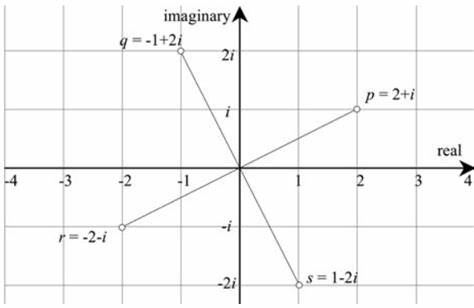
\includegraphics[width=0.6\textwidth]{figures/chapter3/ArgandDiagram.png} 
    \caption{复平面}
    \label{fig:ArgandDiagram}
\end{figure}
\vspace{1em}

\begin{definition}[复数的三角式]
    复平面上一点用极坐标表示:
    \[
        \left\{\begin{array}{l} x=\rho \cos \varphi \\ y=\rho \sin \varphi \end{array}\right.
    \]
    得到复数的三角式:
    \begin{equation}
        z = x + yi = \rho (\cos \varphi + i \sin \varphi)
        \label{eq:ComplexPolar}
    \end{equation}
    其中,
    \begin{enumerate}
        \item $\rho = |z| = \sqrt{x^2 + y^2}$ 为复数的模(Modulus);
        \item $\varphi = \arg z$ 为复数的辐角(Argument),既正实轴到复数向量的逆时针夹角。一个复数的幅角值不能唯一确定,可以取无穷多个值,并且彼此相差 $2k\pi,\ k\in\mathbb{Z}$。
    \end{enumerate}
\end{definition}

\begin{figure}[htbp]
    \centering
    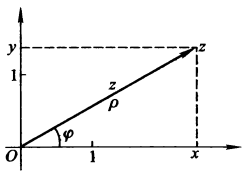
\includegraphics[width=0.4\textwidth]{figures/chapter3/chapter3_4_2} 
    \caption{复数的三角式}
    \label{fig:ComplexPolar}
\end{figure}
\vspace{1em}

\begin{theorem}[复数乘法的三角式]
    设 $z_1=\rho_1(\cos\varphi_1 + i\sin\varphi_1),\ z_2=\rho_2(\cos\varphi_2 + i\sin\varphi_2)\in\mathbb{C}$,则
    \[
        z_1 z_2 = \rho_1 \rho_2 [\cos(\varphi_1 + \varphi_2) + i \sin(\varphi_1 + \varphi_2)]
    \]
\end{theorem}

\begin{corollary}[棣莫弗公式 De Moivre's Theorem]
    设 $z=\rho(\cos\varphi + i\sin\varphi)\in\mathbb{C}$,$n\in\mathbb{Z}$,则
    \begin{equation}
        z^n = \rho^n [\cos(n\varphi) + i \sin(n\varphi)]
        \label{eq:DeMoivreTheorem}
    \end{equation}
\end{corollary}
\vspace{1em}
\begin{note}
    通过复数的三角式,说明复数乘法的几何意义:两个复数相乘,模相乘,幅角相加。将 $z_1$ 的长度拉伸 $\rho_2$ 倍,并逆时针旋转 $\varphi_2$ 角度,得到 $z_1 z_2$。
\end{note}
\vspace{1em}

\subsection{复数的指数式}

\begin{theorem}[欧拉公式 Euler's Formula]
    设 $\theta\in\mathbb{R}$,则
    \begin{equation}
        e^{i\theta} = \cos\theta + i\sin\theta
        \label{eq:EulerFormula}
    \end{equation}
\end{theorem}
\vspace{1em}

\begin{definition}[复数的指数式]
    将欧拉公式 \ref{eq:EulerFormula} 代入复数的三角式 \ref{eq:ComplexPolar},得到复数的指数式:
    \begin{equation}
        z = \rho e^{i\varphi}
        \label{eq:ComplexExponential}
    \end{equation}
    其中,$\rho = |z|$ 为复数的模,$\varphi = \arg z$ 为复数的辐角。
\end{definition}

\begin{theorem}[复数乘法的指数式]
    设 $z_1=\rho_1 e^{i\varphi_1},\ z_2=\rho_2 e^{i\varphi_2}\in\mathbb{C}$,则
    \[
        z_1 z_2 = \rho_1 \rho_2 e^{i(\varphi_1 + \varphi_2)}
    \]
\end{theorem}

% \begin{theorem}[复数的幂运算]
%     设 $z=\rho e^{i\varphi}\in\mathbb{C}$,$p\in \mathbb{C}$,则
%     \[
%         z^p = \rho^p e^{ip\varphi}
%     \]
% \end{theorem}

\begin{theorem}[复数除法的指数式]
    设 $z_1=\rho_1 e^{i\varphi_1},\ z_2=\rho_2 e^{i\varphi_2}\in\mathbb{C},\ z_2\neq 0$,则
    \[
        \frac{z_1}{z_2} = \frac{\rho_1}{\rho_2} e^{i(\varphi_1 - \varphi_2)}
    \]
\end{theorem}

\newpage